\documentclass[10pt]{article}
\usepackage[a4paper,margin=1.8cm]{geometry}
\usepackage{fontspec}\setmainfont{texgyretermes}[Extension=.otf,UprightFont=*-regular,BoldFont=*-bold,ItalicFont=*-italic,BoldItalicFont=*-bolditalic]
\usepackage{enumitem,titlesec,graphicx}
\setlist{nosep,leftmargin=1.2em}
\titleformat{\section}{\normalsize\bfseries}{}{0pt}{}\titlespacing*{\section}{0pt}{6pt}{2pt}
\pagestyle{empty}
\begin{document}
\begin{center}
{\large\bfseries Accurate pressure, wrong flow: downstream errors of Darcy neural operators}\\[2pt]
Aryamann Srivastava, Varun Sathaye, Atishay Jain, Vedant S. Tiwari, IIT Kanpur
\end{center}

\section{Research gap}
Neural operators for steady Darcy flow are trained and ranked on PDEBench by the relative $L^2$ error of the pressure.
Applications use the flux $q=-\kappa\nabla u$: effective permeability, travel times, transport. No published work tests
whether pressure accuracy carries over to these quantities, or which training choices make it do so. Related work stops
short: FlowGuard (2026) re-solves the PDEBench labels but scores pressure only; Boon et al.\ (2023) show flux and pressure
errors diverge for reduced-order Darcy models, not neural operators; Chakraborty and Chen (2026) show better field scores
can mean worse physics, for airfoils; Sobolev and $H^1$ training (Zhang et al.\ 2026) is not evaluated on flux or
downstream quantities.

\section{How we fill it}
\begin{enumerate}
\item \textbf{Converged references.} Re-solve the PDEBench $128^2$ split with a self-converged finite-volume solver
(0.06\% from $256^2$ to $512^2$). The published labels deviate by 5.8\% on average (boundary convention plus
non-convergence), confirming FlowGuard; all models are trained and scored on converged labels.
\item \textbf{Flux metric.} Conservative two-point face fluxes and the interface band (cells within two of a permeability jump).
\item \textbf{Downstream metrics.} A pressure-drop problem on the same maps; from each predicted pressure we compute the
effective permeability $k_{\mathrm{eff}}$ and flux-weighted breakthrough times by semi-analytical (Pollock) particle tracking.
\item \textbf{Controlled comparison.} FNO, U-Net, DeepONet; $L^2$, $H^1$ and a permeability-weighted face-flux loss;
three seeds; in-distribution and shifted test sets (contrast, phase count, roughness, permeability level).
\end{enumerate}

\section{Findings so far}
\begin{itemize}
\item FNO and U-Net with 0.33\% and 0.23\% pressure error have 8.9\% and 5.4\% flux error, concentrated at permeability jumps.
\item With the $L^2$ loss, 0.2\% pressure error gives 9 to 14\% $k_{\mathrm{eff}}$ error, and FNO and U-Net swap rank
between pressure and $k_{\mathrm{eff}}$.
\item $H^1$ gives the best pressure but 3.5 to 6.2\% $k_{\mathrm{eff}}$ error. The face-flux loss gives at most 1.3\%
$k_{\mathrm{eff}}$ and at most 2.4\% late-breakthrough error at the same pressure error, with no architecture change.
\item On maps from an independent generator: 11 to 23\% $k_{\mathrm{eff}}$ error with the face-flux loss, 53 to 894\% otherwise.
\end{itemize}
\begin{center}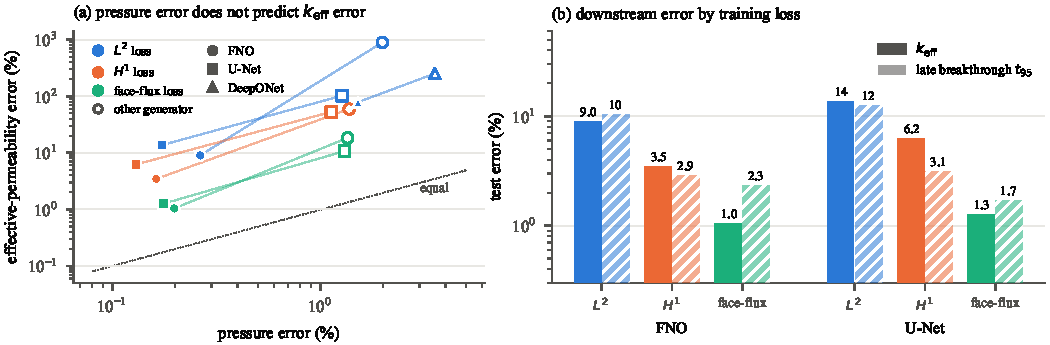
\includegraphics[width=0.95\textwidth]{fig_drop.pdf}\end{center}

\section{Novelty}
First measurement of how pressure error in Darcy neural operators translates into flux, effective-permeability and
breakthrough-time error against converged references, and first comparison of training losses on those quantities.
The label re-solve builds on FlowGuard; the scaling normalisation used for shifted permeability levels is from
Neural Green's Operators (2026). Neither is claimed as new.

\section{Why it matters}
Surrogates are adopted for upscaling, groundwater and reservoir screening, where $k_{\mathrm{eff}}$ and arrival times are
the outputs. A model chosen by pressure error can be the worse one for these uses. We give the community converged labels,
a downstream benchmark and a one-line loss change, and propose flux and downstream errors as standard metrics.
Target: ERCOFTAC ML4Fluids workshop, Florence, April 2027 (abstract due 4 December 2026).
\end{document}
